El sprint A empieza el día Viernes 26 de Septiembre del 2014. Este sprint consta de 2 semanas para completar las historias que serán definidas en la planificación del sprint. El sprint concluirá el Jueves 9 de Octubre del 2014.

%\begin{landscape}
\subsection{Sprint backlog}
En este sprint se eligió trabajar en los features 1 y 2 del product backlog, por el hecho de tener alta prioridad.  Cada feature se divide en historias de usuario, y estas son estimadas con puntos de historia. En los Cuadros \ref{table:eus1} y \ref{table:eus2} se definen las estimaciones. Para cada historia de usuario se definen criterios de aceptación, como se muestra en el Cuadro~\ref{table:criteriosSA}.

Cada historia de usuario se divide en tareas, y se definen en los Cuadros \ref{table:tareasUS1}, \ref{table:tareasUS2} y \ref{table:tareasUS3_1}.

%--------------------------------------------------------------------
\begin{table}[ht]
\centering
\begin{tabular}{|l|p{6cm}|c|p{5cm}|r|}
\hline
\textbf{No.} & \textbf{Feature} & \textbf{Id.} & \textbf{Historia de usuario} & \textbf{Estimación} \\
\hline
1 & \pbrecon & US1 & Obtener coordenadas de objetos reconocidos. & 3 \\ 
\hline
\end{tabular}
\caption{Estimación de US1}
\label{table:eus1}
\end{table}

%--------------------------------------------------------------------
\begin{table}[ht]
\centering
\begin{tabular}{|l|p{6cm}|c|p{5cm}|r|}
\hline
\textbf{No.} & \textbf{Feature} & \textbf{Id.} & \textbf{Historia de usuario} & \textbf{Estimación} \\
\hline
2 & \multirow{2}{6cm}{\pbprof} 
& US2 & Controlar la posición de la cámara. & 3 \\
\cline{3-5}
& & US3 & Obtener distancia aproximada de los objetos reconocidos. & 8 \\
\hline
\end{tabular}
\caption{Estimación de US2 y US3}
\label{table:eus2}
\end{table}


%--------------------------------------------------------------------
\begin{table}[ht]
\centering
\begin{tabular}{|l|p{15cm}|}
\hline
\textbf{Id.} & \textbf{Criterios de aceptación}\\
\hline
US1 & El software a implementar debe ser capaz de reconocer las coordenadas de un objeto en tiempo real, pueden ser de uno o varios objetos captados en el fotograma. \\
\hline
US2 & Dando como entrada el ángulo con respecto al eje vertical, la cámara debe ser capaz de posicionarse al ángulo de entrada establecido. \\
\hline
US3 & Ya teniendo las coordenadas del objeto, el software a implementar debe ser capaz de devolver la distancia que existe entre un objeto y el robot. \\
\hline
\end{tabular}
\caption{Criterios de aceptación del sprint A}
\label{table:criteriosSA}
\end{table}


%--------------------------------------------------------------------
\begin{table}[ht]
\centering
\begin{tabular}{|c|p{13cm}|}
\hline
\textbf{US1} & \textbf{Obtener coordenadas de objetos reconocidos} \\
\hline
\hline
\textbf{Id.} & \textbf{Tareas}\\
\hline
T1 & Preparar estructura simple de archivos para el sistema  \\ \hline
T2 & Investigar acerca OpenCV \\ \hline
T3 & Configurar e instalar OpenCV en Raspberry Pi y en la laptop de trabajo \\ \hline
T4 & Investigar acerca de OpenCVBlobsLib \\ \hline
T5 & Investigar acerca de filtros de OpenCV para el POC \\ \hline
T6 & Implementar POC usando OpenCVBlobsLib \\ \hline
T7 & Escribir función que devuelva coordenadas de los blobs identificados \\ \hline
T8 & Hacer pruebas de la implementación en Raspberry Pi \\ \hline
\end{tabular}
\caption{Tareas del US1}
\label{table:tareasUS1}
\end{table}

%--------------------------------------------------------------------
\begin{table}[ht]
\centering
\begin{tabular}{|c|p{13cm}|}
\hline
\textbf{US2} & \textbf{Controlar la posición de la cámara.} \\
\hline
\hline
\textbf{Id.} & \textbf{Tareas} \\
\hline
T1 & Fabricar soporte motorizado para cámara \\ \hline
T2 & Implementar función que gira la cámara a una posición especifica \\ \hline
T3 & Escribir y ejecutar prueba de unidad para el método que gira la cámara \\ \hline
\end{tabular}
\caption{Tareas del US2}
\label{table:tareasUS2}
\end{table}


%--------------------------------------------------------------------
\begin{table}[ht]
\centering
\begin{tabular}{|c|p{13cm}|}
\hline
\textbf{US3} & \textbf{Obtener distancia aproximada de los objetos reconocidos} \\
\hline
\hline
\textbf{Id.} & \textbf{Tareas} \\
\hline
T1 & Deducir fórmulas para obtener la distancia de los objetos en la pantalla, de acuerdo con el ángulo de inclinación de la cámara. \\ \hline
T2 & Implementar función que devuelva distancia de objetos. \\ \hline
\end{tabular}
\caption{Tareas del US3}
\label{table:tareasUS3_1}
\end{table}
%--------------------------------------------------------------------

\subsection{Reconocimiento de objetos utilizando OpenCV}\label{sec:recopencv}
El sistema de reconocimiento de objetos ejecuta una serie de pasos antes de enviar un fotograma al reconocimiento de blobs. Primero se ejecuta \texttt{dilate()}, para remover pequeños puntos en la imagen, que no son relevantes para este caso. Segundo se ejecuta \texttt{Canny()}, que devuelve una imagen con bordes delgados y finos. Una vez ejecutados estos pasos se envía la imagen resultado a \texttt{CBlobresult()}, que devuelve los blobs detectados en la imagen. Todo este proceso se puede apreciar en la Figura~\ref{fig:opencvproc}.

El resultado de \texttt{CBlobresult()} es un conjunto de blobs. Cada elemento del conjunto contiene datos como ser: el área, coordenadas de la posición, dimensiones, etc. 
%Algunos datos de este conjunto de blobs resultado es enviado al sistema experto como datos de entrada.

\begin{figure}
  \centering
    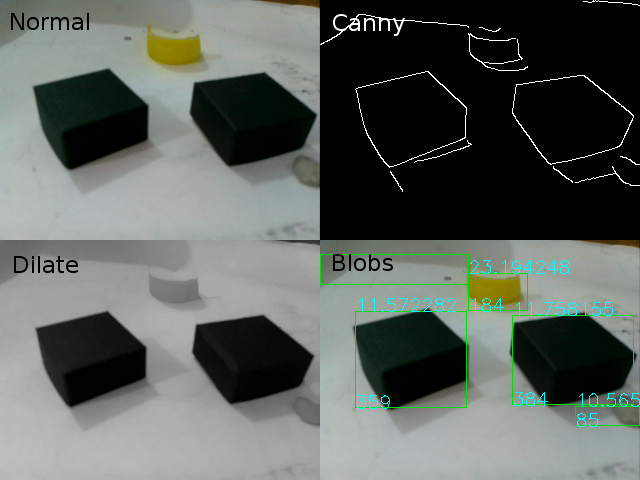
\includegraphics[width=0.5\textwidth]{opencvproc}
  \caption{Reconocimiento de objetos utilizando OpenCV. Elaboración propia.}
  \label{fig:opencvproc}
\end{figure}

\subsection{Control del servomotor de la cámara}
La cámara estará montada a un servomotor y este al robot, de manera que será posible mover la cámara en el eje vertical como se muestra en la Figura~\ref{fig:servo}.

\begin{figure}
  \centering 
    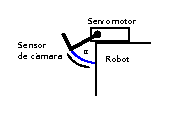
\includegraphics[width=0.5\textwidth]{servo}
  \caption{Cámara y servomotor montados al Robot. Elaboración propia.}
  \label{fig:servo}
\end{figure}
%https://github.com/richardghirst/PiBits/tree/master/ServoBlaster
Ya teniendo al servomotor y a la cámara montados, es necesario poder controlarlos. El servomotor recibe números para poder moverlo, la forma de poder enviar números es mediante un archivo especial llamado \texttt{/dev/servoblaster}. ServoBlaster es una interfaz para controlar servomotores mediante los pines de GPIO. Los números que recibe ServoBlaster son ancho de pulsos, luego estos datos son transmitidos mediante el GPIO hasta el servomotor. Para poder mover la cámara a un cierto ángulo con respecto al eje vertical, es necesario transformar los anchos de pulsos a grados, para esta transformación se utilizará la técnica de interpolación de Lagrange \cite{ipolinomica}.

\begin{equation}
p(x) = \sum_{i=0}^{n}\left(\prod_{\substack{0 \leq j \leq n \\ j \neq i}}{\frac{x - x_j}{x_i - x_j}}\right) * y_i \label{lagrange}
\end{equation}

Se utilizaran tres puntos, que cada uno es el ángulo en grados (con respecto al eje vertical como se muestra en la Figura~\ref{fig:servo}) con su correspondiente ancho de pulso. Estos puntos se muestran en el Cuadro~\ref{table:puntosg2pwm}.

\begin{table}
\centering
\begin{tabular}{| r | r | r |}
\hline
  & \textbf{x} & \textbf{y} \\
\hline
0 & 180 & 89 \\ 
\hline
1 &  90 & 189 \\
\hline
2 &  45 & 242 \\
\hline
\end{tabular}
\caption{Conversión de grados a modulación por ancho de pulso}
\label{table:puntosg2pwm}
\end{table}

Luego reemplazando en \ref{lagrange} se obtiene la Ecuación~\ref{servolagr}.

%p(x) =  \frac{(x - 90) * (x - 45)}{12150} * 89 + \\
%        \frac{(x - 180) * (x - 45)}{-4050} * 189 + \\
%        \frac{(x - 180) * (x - 90)}{-6075} * 242 \label{servolagr}

\begin{equation}
p(x) = \frac{(x - x_1) * (x - x_2) * y_0}{(x_0 - x_1) * (x_0 - x_2)} + \frac{(x - x_0) * (x - x_2) * y_1}{(x_1 - x_0) * (x_1 - x_2)} + \frac{(x - x_0) * (x - x_1) * y_2}{(x_2 - x_0) * (x_2 - x_1)} \label{servolagr} 
\end{equation}

En la Ecuación~\ref{servolagr}, $x$ representa el ángulo de entrada, y el resultado de $p(x)$ es el ancho de pulso. Con este dato ya es posible indicar al servomotor cuanto se debe mover para posicionar la cámara al ángulo $x$, que seria $\alpha$ en la Figura~\ref{fig:servo}.

\subsection{Casos de prueba}


\begin{longtable}{|l|p{10cm}|}
\hline
\textbf{Id.} & CP1 \\
\hline
\textbf{Historia} & US1\\
\hline
\textbf{Nombre} & Prueba de funcionamiento de ambiente de desarrollo \\
\hline
\textbf{Descripción} & Se realizarán pruebas de OpenCV de los ambientes de desarrollo de Raspberry Pi, para verificar que OpenCV y las herramientas de desarrollo estén correctamente instaladas \\
\hline
\textbf{Ambiente de prueba} & Raspberry Pi con Raspbian y OpenCV \\
\hline
\textbf{Inicialización} & Encender Raspberry Pi\\
\hline
%\textbf{Finalización} & Ninguna\\
%\hline
\textbf{Acciones} &  
\parbox[][][s]{8cm}{ 
            \begin{itemize}
                \item Copiar \texttt{opencv-2.4.9.zip} al Raspberry Pi
                \item Descomprimir \texttt{opencv-2.4.9.zip}
                \item Entrar a opencv-2.4.9/samples/cpp
                \item Ejecutar \texttt{\$ g++ `pkg-config --libs --cflags opencv` houghlines.cpp -o houghlines}
                \item Ejecutar \texttt{./houghlines}
            \end{itemize} 
}
\\
\hline
\textbf{Salida esperada} & Dos ventanas gráficas con títulos ``source'' y ``detected lines''. La segunda ventana tiene los bordes marcados con rojo.\\
\hline
\textbf{Salida obtenida} & En la Figura~\ref{fig:houghlinesRes} se muestra la salida obtenida de Houghlines, que es una transformada usada para detectar lineas rectas. \\
\hline
\textbf{Resultado} & \textbf{Correcto}\\
\hline
\end{longtable}

\begin{figure}
  \centering
    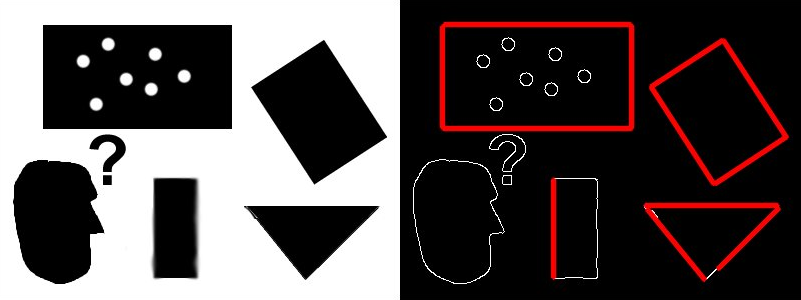
\includegraphics[width=0.5\textwidth]{houghlines}
  \caption{Salida de ejecución de Houghlines. Elaboración propia.}
  \label{fig:houghlinesRes}
\end{figure}

%----------------------

\begin{longtable}{|l|p{10cm}|}
\hline
\textbf{Id.} & CP2 \\
\hline
\textbf{Historia} & US1\\
\hline
\textbf{Nombre} & Prueba de funcionamiento de ambiente de desarrollo en laptop de trabajo \\
\hline
\textbf{Descripción} & Se realizarán pruebas de OpenCV de los ambientes de desarrollo de la laptop de trabajo, para verificar que OpenCV y las herramientas de desarrollo estén correctamente instaladas. \\
\hline
\textbf{Ambiente de prueba} & Laptop de trabajo y OpenCV \\
\hline
\textbf{Inicialización} & Ninguna\\
\hline
%\textbf{Finalización} & Ninguna\\
%\hline
\textbf{Acciones} &  
\parbox[][][s]{8cm}{ 
            \begin{itemize}
                \item Encender laptop y entrar a la terminal.
                \item Copiar \texttt{opencv-2.4.9.zip} a directorio.
                \item Descomprimir \texttt{opencv-2.4.9.zip}
                \item Entrar a opencv-2.4.9/samples/cpp
                \item Ejecutar \texttt{\$ g++ `pkg-config --libs --cflags opencv` houghlines.cpp -o houghlines}
                \item Ejecutar \texttt{./houghlines}
            \end{itemize} 
}
\\
\hline
\textbf{Salida esperada} & Dos ventanas gráficas con títulos ``source'' y ``detected lines''. La segunda ventana tiene los bordes marcados con rojo.\\
\hline
\textbf{Salida obtenida} & En la Figura~\ref{fig:houghlinesLap} se muestra la salida obtenida de Houghlines, que es una transformada usada para detectar lineas rectas.\\
\hline
\textbf{Resultado} & \textbf{Correcto}\\
\hline
\end{longtable}

\begin{figure}
  \centering
    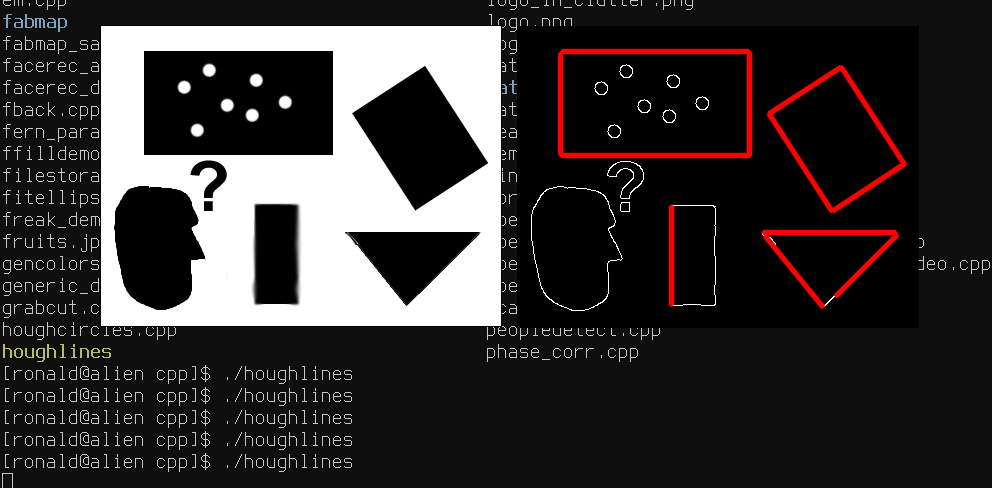
\includegraphics[width=0.5\textwidth]{houghlinesLap}
  \caption{Salida de ejecución de Houghlines. Elaboración propia.}
  \label{fig:houghlinesLap}
\end{figure}

%---------------------------

\begin{longtable}{|l|p{10cm}|}
\hline
\textbf{Id.} & CP3 \\
\hline
\textbf{Historia} & US1\\
\hline
\textbf{Nombre} & Prueba de funcionamiento de \texttt{Blobs::findBlobs} \\
\hline
\textbf{Descripción} & Se realizarán pruebas de \texttt{Blobs::findBlobs}, para verificar que este método encuentra regiones (blobs) en una imagen dada. \\
\hline
\textbf{Ambiente de prueba} & Computadora con OpenCV, herramientas de desarrollo y código fuente del proyecto. \\
\hline
\textbf{Inicialización} & Ninguna \\
\hline
%\textbf{Finalización} & Ninguna \\
%\hline
\textbf{Acciones} &  
\parbox[][][s]{8cm}{ 
            \begin{itemize}
                \item Ingresar a la computadora de desarrollo
                \item Ir al directorio sistema/unit\_tests
                \item Ejecutar la compilación de la prueba de unidad: \texttt{\$ make test\_find\_blobs}
                \item El anterior paso debería generar test\_find\_blobs
                \item Ejecutar \texttt{./test\_find\_blobs}
            \end{itemize} 
}
\\
\hline
\textbf{Salida esperada} & Una ventana gráfica con una foto de tres objetos negros, cada objeto con un recuadro verde.\\
\hline
\textbf{Salida obtenida} & En la Figura~\ref{fig:testBlobsRes} se muestra la salida obtenida. El método \texttt{GetNumBlobs()} usado aquí, se ocupa de detectar objetos en una imagen dada.\\
\hline
\textbf{Resultado} & \textbf{Correcto}\\
\hline
\end{longtable}

\begin{figure}
  \centering
    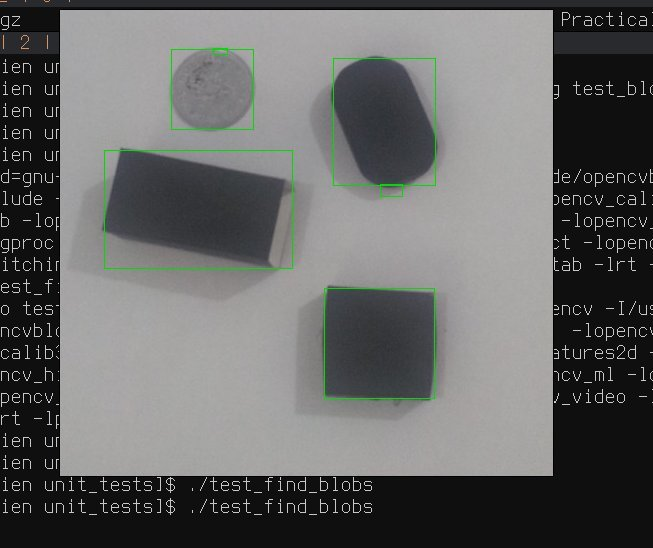
\includegraphics[width=0.5\textwidth]{testBlobsRes}
  \caption{Salida de ejecución de \texttt{./test\_find\_blobs}.  Elaboración propia.}
  \label{fig:testBlobsRes}
\end{figure}

%---------------------------

\begin{longtable}{|l|p{10cm}|}
\hline
\textbf{Id.} & CP4 \\
\hline
\textbf{Historia} & US1\\
\hline
\textbf{Nombre} & Prueba de funcionamiento de coordenadas de \texttt{Blobs::findBlobs} \\
\hline
\textbf{Descripción} & Se realizarán pruebas para verificar que las coordenadas que devuelve \texttt{Blobs::findBlobs} sean correctas \\
\hline
\textbf{Ambiente de prueba} & Computadora con OpenCV, herramientas de desarrollo, código fuente del proyecto, y GIMP \\
\hline
\textbf{Inicialización} & Ninguna \\
\hline
%\textbf{Finalización} & Ninguna \\
%\hline
\textbf{Acciones} &  
\parbox[][][s]{8cm}{ 
            \begin{itemize}
                \item Ingresar a la computadora de desarrollo
                \item Ir al directorio sistema/unit\_tests
                \item Ejecutar la compilación de la prueba de unidad: \texttt{\$ make test\_find\_blobs}
                \item El anterior paso debería generar test\_find\_blobs
                \item Ejecutar \texttt{./test\_find\_blobs}
                \item Verificar que todas las coordenadas listadas en la salida del programa sean las mismas que los recuadros verdes. Esto se puede realizar con la ayuda de GIMP.
            \end{itemize} 
}
\\
\hline
\textbf{Salida esperada} & Salida en la interfaz de linea de comandos con las coordenadas marcadas en la ventana gráfica. En esta ventana debe mostrar una foto de tres objetos negros, cada objeto con un recuadro verde. (Es posible que se muestren otros recuadros verdes en otras regiones, esto es completamente normal.)\\
\hline
\textbf{Salida obtenida} & En la Figura~\ref{fig:test_blob_coord} se muestra la salida obtenida. El método \texttt{GetNumBlobs()} también devuelve las coordenadas de los objetos detectados (blobs).\\
\hline
\textbf{Resultado} & \textbf{Correcto}\\
\hline
\end{longtable}

\begin{figure}
  \centering
    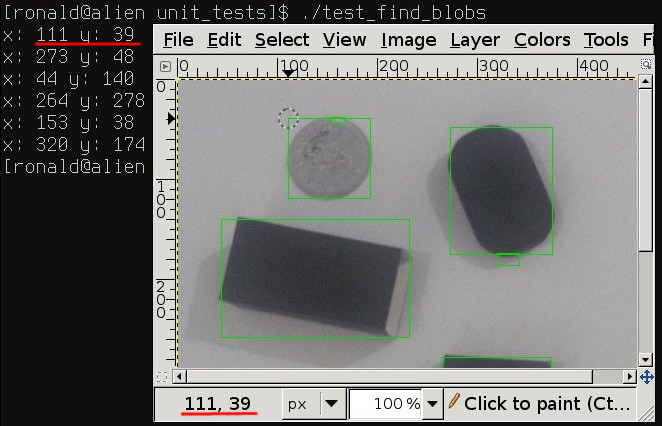
\includegraphics[width=0.5\textwidth]{test_blob_coord}
  \caption{Salida de \texttt{./test\_find\_blobs} mostrando las coordenadas de los blobs. Elaboración propia.}
  \label{fig:test_blob_coord}
\end{figure}


%---------------------------

\begin{longtable}{|l|p{10cm}|}
\hline
\textbf{Id.} & CP5 \\
\hline
\textbf{Historia} & US2\\
\hline
\textbf{Nombre} & Prueba de posicionamiento de la cámara\\
\hline
\textbf{Descripción} & Se realizarán pruebas para verificar que la cámara este correctamente posicionada según el software implementado. \\
\hline
\textbf{Ambiente de prueba} & Raspberry Pi con OpenCV, cámara de Raspberry Pi, herramientas de desarrollo, código fuente del proyecto, y un transportador. \\
\hline
\textbf{Inicialización} & Conectar la cámara a Raspberry Pi. Marcar una hoja desde 40 grados hasta 180 grados.\\
\hline
%\textbf{Finalización} & Ninguna\\
%\hline
\textbf{Acciones} &  
\parbox[][][s]{8cm}{ 
            \begin{itemize}
                \item Ingresar al Raspberry Pi
                \item Ir al directorio sistema/unit\_tests
                \item Ejecutar la compilación de la prueba de unidad: \texttt{\$ make test\_servo}
                \item Verificar que el anterior paso genero test\_servo
                \item Ejecutar \texttt{./test\_servo}
                \item Con la hoja marcada, verificar que la cámara este correctamente alineada según los grados que se muestran en la pantalla.
            \end{itemize} 
}
\\
\hline
\textbf{Salida esperada} & Los grados de la hoja deben coincidir con los grados mostrados en la salida del programa.\\
\hline
\textbf{Salida obtenida} & En la Figura~\ref{fig:test_camara_calib} se muestra la salida obtenida. En la figura se puede obsevar a la cámara alineada a 90 grados.\\
\hline
\textbf{Resultado} & \textbf{Correcto}\\
\hline
\end{longtable}

\begin{figure}
  \centering
    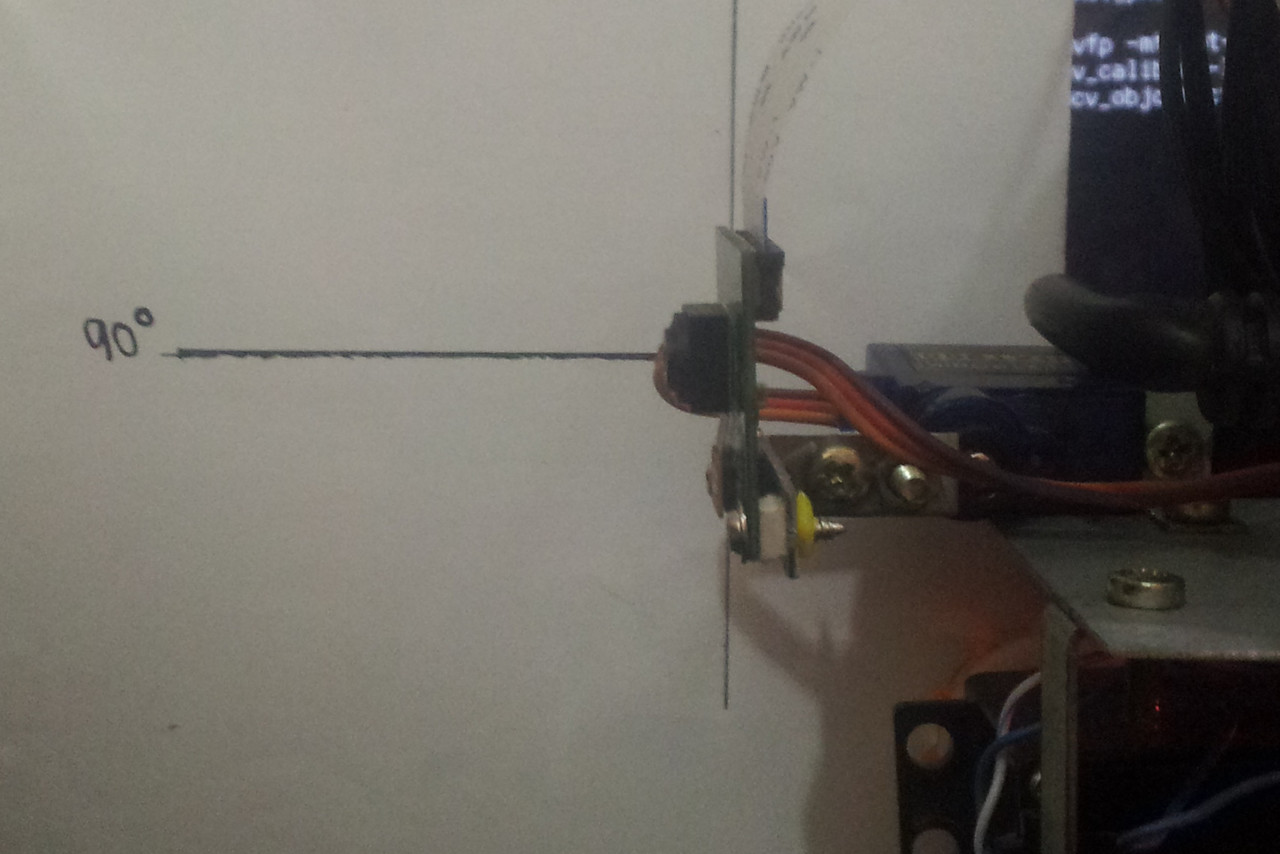
\includegraphics[width=0.5\textwidth]{test_camara_calib}
  \caption{Cámara alineada a 90 grados. Elaboración propia.}
  \label{fig:test_camara_calib}
\end{figure}

\subsection{Demostración de fin de sprint}
 
El método \texttt{findBlobs()} encuentra blobs en una imagen dada (\texttt{im}). En la Figura~\ref{fig:test_blob_coord} se observa las coordenadas de los objetos reconocidos.

\begin{lstlisting}[label=findBlobs,caption=Método para encontrar blobs en una imagen]
CBlobResult Blobs::findBlobs(Mat im){
    Mat img, imgc, imgd;

    cvtColor(im,img,CV_BGR2GRAY);
    Mat st_elem = getStructuringElement(MORPH_RECT, Size(size_slider, size_slider));
    dilate(img, imgd, st_elem);

    Canny(imgd, imgc, canny_th1, canny_th2);

    return CBlobResult(imgc,Mat(),NUMCORES);
}
\end{lstlisting}


El método \texttt{addBlobToImg()} añade un rectángulo al objeto reconocido (blob). Este método recibe como parámetros de entrada, una imagen \texttt{im} y un blob \texttt{t2}. Se obtienen las coordenadas de \texttt{t2} y se utiliza la función \texttt{rectangle} para añadir el rectángulo a la imagen \texttt{im}. En la Figura~\ref{fig:testBlobsRes} se observa que cuatro objetos son reconocidos y encuadrados.


\begin{lstlisting}[label=addBlobToImg,caption=Método para añadir rectangulos a blobs]
Mat Blobs::addBlobToImg(Mat im, CBlob t2){

    Scalar mean, stddev;
        
    Rect bbox = t2.GetBoundingBox();
    rectangle(im,bbox,Scalar(0,220,0),1);
    
    return im;
}

\end{lstlisting}


El método \texttt{mover()} mueve el servomotor a un \texttt{ángulo} de entrada especificado.
\begin{lstlisting}[label=mover,caption=Método para mover un servomotor]
void Servo::mover(double angulo){
    FILE * pFile;

    int servo_a = (int) interpolacion(angulo);
    
    string s = std::to_string(servo_a);
    s = SERVO_NUM + s + "\n";
    const char *cstr = s.c_str();
    
    cout << "Servo: " << s << endl;

    if(enable){
        pFile = fopen (SERVO_FILE, "wb");
        if (pFile != NULL){
            fwrite (cstr , sizeof(char), s.size(), pFile) ;
            fclose (pFile);
        }else{
            cout << "No se puede abrir " << SERVO_FILE << endl;
        }
    }
}
\end{lstlisting}

Utilizando la Ecuación~\ref{servolagr} se implementa el método de \texttt{interpolacion()}.

\begin{lstlisting}[label=interpolacion,caption=Método para transformar de grados a modulación por ancho de pulso.]
double Servo::interpolacion(double x){
    
    double x0 = 180, y0 = 89;
    double x1 = 90, y1 = 189;
    double x2 = 45, y2 = 242;

    double y;

    y = ((x - x1) * (x - x2) * y0)/((x0 - x1) * (x0 - x2)) + 
        ((x - x0) * (x - x2) * y1)/((x1 - x0) * (x1 - x2)) + 
        ((x - x0) * (x - x1) * y2)/((x2 - x0) * (x2 - x1));

    return y;
}

\end{lstlisting}

\subsection{Gráfico burn down del sprint}
La Figura~\ref{fig:sprintA} muestra el gráfico \emph{burn down} del presente sprint.

\begin{figure}
  \centering
    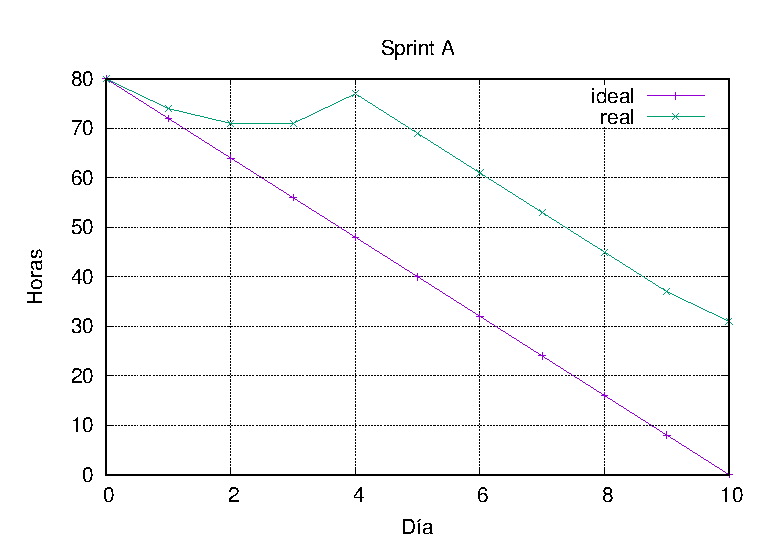
\includegraphics[width=0.5\textwidth]{sprintA}
  \caption{Gráfico burn down del sprint. Elaboración propia.}
  \label{fig:sprintA}
\end{figure}

\subsection{Retrospectiva del sprint}
\begin{itemize}
  \item ¿Qué salió bien?
    \begin{itemize}
        \item Se completaron la mayoria de las tareas de la iteración.
        \item Se escribieron pruebas de unidad para el código desarrollado.
    \end{itemize}

  \item ¿Qué podría haber sido mejor?
    \begin{itemize}
        \item La estimación de la historia US3 no fue buena.
    \end{itemize}

  \item ¿Qué  se puede mejorar en el futuro?
    \begin{itemize}
        \item Mejorar las estimaciones de las historias, si la historia es muy larga es mejor dividirla.
    \end{itemize}
\end{itemize}

